%% GENERATED by tools/from_docs.py from stepss-docs. Do not edit by hand:
%% edit the page named below in stepss-docs and regenerate.
%% source: stepss-docs/src/content/docs/user-guide/eigenanalysis.md

\chapter{Small-signal stability analysis}\label{doc:eigenanalysis}

RAMSES computes small-signal stability analysis internally. It reduces the
linearised differential-algebraic model to a state matrix, solves the dense
eigenproblem, and writes eigenvalues, damping ratios, participation factors and
mode shapes to file. No external tool is involved.

\begin{docsnote}{Requires a RAMSES newer than v3.60}

An older engine accepts the \texttt{EIG} disturbance and writes no results files. The
\texttt{stepss} package version's leading components name the bundled RAMSES, so
\texttt{stepss.\_\_version\_\_} tells you directly.

\end{docsnote}

\section{What is computed}\label{eigenanalysis:what-is-computed}

The linearised model is a set of differential-algebraic equations,

\[
\begin{aligned}
\Delta\dot{x} &= f_x\,\Delta x + f_y\,\Delta y \\
0 &= g_x\,\Delta x + g_y\,\Delta y
\end{aligned}
\]

with states \(x\) and algebraic variables \(y\). Eliminating \(\Delta y\) gives the
state matrix

\[A_{sys} = f_x - f_y\,g_y^{-1}\,g_x\]

whose eigenvalues are the system modes. RAMSES assembles the unreduced Jacobian,
factorises \(g_y\) once with KLU, forms \(A_{sys}\), and solves it with LAPACK.
The elimination exists only if \(g_y\) is nonsingular, which is what makes the
model index-1; a singular \(g_y\) is reported rather than worked around.

For each eigenvalue \(\lambda = \sigma \pm j\omega\):

\begin{small}\begin{longtable}[]{@{}ll@{}}
\toprule\noalign{}
Quantity & Definition \\
\midrule\noalign{}
\endhead
\bottomrule\noalign{}
\endlastfoot
Frequency & \(f = \lvert\omega\rvert / 2\pi\) in Hz \\
Damping ratio & \(\zeta = -\sigma / \lvert\lambda\rvert\) \\
\end{longtable}\end{small}

A mode with \(\zeta < 0\) grows rather than decays: the operating point is
small-signal unstable.

\section{Running an analysis}\label{eigenanalysis:running-an-analysis}

Add an \texttt{EIG} event to the disturbance file:

\begin{Verbatim}
1.000 EIG 'ssa'
\end{Verbatim}

or inject it from Python:

\begin{Verbatim}
import stepss

case = stepss.cfg()
case.addData('lf.dat')
case.addData('dyn.dat')
case.addData('solveroptions.dat')
case.addDst('nothing.dst')
case.addObs('obs.dat')
case.addTrj('out.trj')

ram = stepss.sim()
ram.execSim(case, 0.0)               # pause at the operating point
ram.addDisturb(0.001, "EIG 'ssa'")   # schedule the analysis
ram.contSim(0.01)                    # advance past it so the event fires
ram.endSim()
\end{Verbatim}

Results are computed at the instant the event fires, so where you pause
determines what you get. Small-signal results are only meaningful at an
operating point: pausing mid-swing linearises about a non-equilibrium.

\subsection{Required settings}\label{eigenanalysis:required-settings}

\begin{small}\begin{longtable}[]{@{}
  >{\raggedright\arraybackslash}p{(\linewidth - 4\tabcolsep) * \real{0.2266}}
  >{\raggedright\arraybackslash}p{(\linewidth - 4\tabcolsep) * \real{0.7734}}
@{}}
\toprule\noalign{}
\begin{minipage}[b]{\linewidth}\raggedright
Setting
\end{minipage} & \begin{minipage}[b]{\linewidth}\raggedright
Why
\end{minipage} \\
\midrule\noalign{}
\endhead
\bottomrule\noalign{}
\endlastfoot
\texttt{\$OMEGA\_REF\ SYN} & Under the centre-of-inertia frame the COI equations are computed by finite differences and never enter the assembled Jacobian, so reducing under COI would silently hold COI speed constant and produce a plausible, wrong spectrum \\
\texttt{\$SCHEME\ DE} & Under the integrated scheme the pure differential-algebraic values exist only briefly inside the Newton loop \\
\end{longtable}\end{small}

Both are refused rather than approximated. See \hyperref[eigenanalysis:refusals]{Refusals} below.

One optional setting, \texttt{\$PF\_THRES\ x}, sets the floor below which a participation
entry is not written, default \texttt{1e-3}. It is a size guard on the one output that
is quadratic in the state count, in the same family as \texttt{\$EIG\_MAX\_STATES}, and
not a threshold anyone is meant to tune per analysis; see
\hyperref[eigenanalysis:namepfdat]{\texttt{\textless{}name\textgreater{}\_pf.dat}} below.

They are yours to set on the command line and from Python. The graphical
interface's \textbf{Run small-signal stability analysis} writes both itself, into an
extra data file read after the case's own, so a case configured for time-domain
runs analyses without being edited. Settings are applied in the order they are
read and the last of each kind wins, which is what makes that an override rather
than a conflict.

\section{Output files}\label{eigenanalysis:output-files}

Three files per analysis, named from the basename given to \texttt{EIG}. All are plain
whitespace-separated text with \texttt{\#} comment headers, so \texttt{numpy.loadtxt} reads
them directly. Names are left-justified and contain no spaces, so splitting on
whitespace is safe.

\textbf{All three carry every mode.} Nothing the engine writes decides which modes
are worth looking at; that is the reader's job, and both interfaces filter live
against the full set. The only floor anywhere is \texttt{\$PF\_THRES}, on participation
alone, and its reason is size rather than significance.

The first line of each file is a version banner, and these three are at \textbf{v2}.

\subsection{\texorpdfstring{\texttt{\textless{}name\textgreater{}\_modes.dat}}{\textless name\textgreater\_modes.dat}}\label{eigenanalysis:name_modes.dat}

One line per mode, every mode written.

\begin{small}\begin{longtable}[]{@{}ll@{}}
\toprule\noalign{}
Column & Meaning \\
\midrule\noalign{}
\endhead
\bottomrule\noalign{}
\endlastfoot
\texttt{index} & Mode number, 1-based \\
\texttt{re}, \texttt{im} & Real and imaginary parts of \(\lambda\) \\
\texttt{zeta} & Damping ratio \\
\texttt{freq\_hz} & Frequency in Hz \\
\texttt{smp} & 1 if the eigenvalue is simple, 0 if degenerate \\
\end{longtable}\end{small}

The header records \texttt{nstates}, \texttt{nalg}, the time, \texttt{gap\_tol}, and \texttt{pf\_floor}, the
participation floor the run applied.

\begin{docsnote}{Reading a v1 file}

v1 carried a \texttt{dom} column between \texttt{freq\_hz} and \texttt{smp}, holding the engine's
verdict on whether the mode passed the \texttt{real\_limit} it was given, and recorded
\texttt{real\_limit} and \texttt{pf\_threshold} in the header instead of \texttt{pf\_floor}. The two
layouts have the same field widths, so a reader that ignores the banner does
not fail on the wrong one: it reads \texttt{smp} out of the \texttt{dom} column and answers
wrongly. Check the first line.

\end{docsnote}

\subsection{\texorpdfstring{\texttt{\textless{}name\textgreater{}\_pf.dat}}{\textless name\textgreater\_pf.dat}}\label{eigenanalysis:name_pf.dat}

Participation factors, one line per mode and state:
\texttt{mode}, \texttt{state}, \texttt{pf}, \texttt{family}, \texttt{device}, \texttt{variable}. The \texttt{pf} column is the
participation factor itself, which STEPSS GUI abbreviates to \textbf{PF}.

The participation of state \(k\) in mode \(i\) is \(p_{ki} = \lvert w_{ki}\,v_{ki}\rvert\),
built from the left and right eigenvectors and normalised so each mode's largest
entry is 1.

Written for every mode, and for every entry above
\hyperref[ch-settings]{\texttt{\$PF\_THRES}}, so a state that is absent is below
that floor rather than exactly zero. This is the one output quadratic in the
state count: one row per (mode, state) pair, so at the \texttt{\$EIG\_MAX\_STATES} ceiling
of 5000 states an unfloored file would be 25 million rows and roughly 2 GB,
nearly all of it entries too small to read. At the default the same run writes
on the order of a hundred thousand.

\textbf{No mode can be emptied by the floor} for any value below 1, because
normalisation puts one entry at exactly 1 in every mode. Raise it to bound the
file on a large system; lower it to see smaller entries.

\subsection{\texorpdfstring{\texttt{\textless{}name\textgreater{}\_ms.dat}}{\textless name\textgreater\_ms.dat}}\label{eigenanalysis:name_ms.dat}

Mode shapes, one line per mode and machine:
\texttt{mode}, \texttt{state}, \texttt{magnitude}, \texttt{angle\_deg}, \texttt{device}.

Rotor-speed components for every mode, normalised so the largest magnitude in
each mode is 1, with \textbf{angles relative to that largest entry}, because an
eigenvector's absolute phase is arbitrary. No floor applies: this carries one
row per machine per mode, which is linear in the state count rather than
quadratic.

\section{Saving a run as one archive}\label{eigenanalysis:saving-a-run-as-one-archive}

The three files above are only useful together, and a spectrum is only worth
much beside the matrix it was reduced from. \textbf{STEPSS GUI} writes all of
them, plus the Jacobian that the \hyperref[ch-disturb]{\texttt{JAC}
disturbance} dumped at the
same instant, into a single \texttt{.zip} or \texttt{.tar.gz}: \textbf{Save dynamic Jacobian\ldots{}} on
the Analysis tab, with the format chosen in the dialog. \textbf{Load dynamic
Jacobian\ldots{}} beside it opens one back into a results window of its own, leaving
any window already up alone, so an archived run and a fresh one can be read side
by side.

\begin{small}\begin{longtable}[]{@{}
  >{\raggedright\arraybackslash}p{(\linewidth - 4\tabcolsep) * \real{0.4599}}
  >{\raggedright\arraybackslash}p{(\linewidth - 4\tabcolsep) * \real{0.5401}}
@{}}
\toprule\noalign{}
\begin{minipage}[b]{\linewidth}\raggedright
In the archive
\end{minipage} & \begin{minipage}[b]{\linewidth}\raggedright
\end{minipage} \\
\midrule\noalign{}
\endhead
\bottomrule\noalign{}
\endlastfoot
\texttt{stepss-ssa.txt} & The manifest: the basename, the engine version and \texttt{t} (older archives also carry the \texttt{real\_limit} and \texttt{pf\_threshold} their run was given) \\
\texttt{\textless{}name\textgreater{}\_modes.dat}, \texttt{\textless{}name\textgreater{}\_pf.dat}, \texttt{\textless{}name\textgreater{}\_ms.dat} & The results above \\
\texttt{\textless{}name\textgreater{}\_eqs.dat}, \texttt{\textless{}name\textgreater{}\_var.dat}, \texttt{\textless{}name\textgreater{}\_val.dat}, \texttt{\textless{}name\textgreater{}\_struc.dat} & The unreduced Jacobian \\
\end{longtable}\end{small}

\textbf{An archive is a record of a result, not an input that reproduces one.} The
data files, the solver settings and the disturbance that produced the run are
not in it. It is something to hand to a colleague, attach to an issue, or come
back to in a year and still be able to read; re-running the analysis needs the
case, which is a separate thing to keep.

The manifest is what makes it readable that much later. None of the results
files records which engine wrote them, so an archive analysed by an older build
is otherwise indistinguishable from one made today: STEPSS names the recorded
version when it opens one, and says so when it differs from the engine now in
use. An archive carrying no manifest is refused with a reason rather than opened
into an empty window.

Both formats are ordinary archives that \texttt{unzip} and \texttt{tar\ xzf} read, and
everything sits under one directory named for the run. The archive is also the
only way back into the interface: results sitting loose in a directory, from a
run made at a terminal for instance, are read by the Python API rather than by
STEPSS GUI, which opens a run either by producing it or by loading one of these.

\section{\texorpdfstring{Degenerate modes, and why the \texttt{smp} column matters}{Degenerate modes, and why the smp column matters}}\label{eigenanalysis:degenerate-modes-and-why-the-smp-column-matters}

Identical machine models with identical parameters produce identical poles, so
power system spectra are heavily degenerate. In the Kundur two-area system, 20
of 70 modes share an eigenvalue with another mode.

\textbf{In a degenerate eigenspace the individual eigenvectors are not unique.} The
participation factors and mode shape of such a mode are therefore
basis-dependent: real numbers that carry no physical meaning and that would come
out differently on another LAPACK build.

The \texttt{smp} column is 1 when the gap from this eigenvalue to every other exceeds
\texttt{gap\_tol} (default \texttt{1e-6}, recorded in the header), and 0 otherwise. \textbf{Do not
interpret participation factors or mode shapes for a mode flagged 0.}

\section{Refusals}\label{eigenanalysis:refusals}

The analysis refuses rather than returning a result it cannot justify. Every
refusal writes no results files, states the reason in the log and through
\hyperref[doc:py-api]{\texttt{getLastErr()}}, and exits with code \textbf{78}.

\begin{small}\begin{longtable}[]{@{}
  >{\raggedright\arraybackslash}p{(\linewidth - 4\tabcolsep) * \real{0.3939}}
  >{\raggedright\arraybackslash}p{(\linewidth - 4\tabcolsep) * \real{0.6061}}
@{}}
\toprule\noalign{}
\begin{minipage}[b]{\linewidth}\raggedright
Condition
\end{minipage} & \begin{minipage}[b]{\linewidth}\raggedright
Reason
\end{minipage} \\
\midrule\noalign{}
\endhead
\bottomrule\noalign{}
\endlastfoot
\texttt{\$OMEGA\_REF\ COI} & The assembled Jacobian does not carry the COI equations \\
\texttt{\$SCHEME\ IN} & The pure DAE values are not available at that point \\
States above \texttt{\$EIG\_MAX\_STATES} & The dense solve is not practical at that size \\
Singular \(g_y\) & The model is not index-1 \\
\texttt{EIG} carrying parameters & The record takes a basename and nothing else \\
\end{longtable}\end{small}

That last one is a migration, not a mistake in the usual sense. \texttt{EIG} used to
accept an optional \texttt{real\_limit} and \texttt{pf\_threshold} pair; \texttt{real\_limit} decided
which modes got participation and mode-shape output, and \texttt{pf\_threshold} became
the \texttt{\$PF\_THRES} solver setting. A \texttt{.dst} still carrying them is refused rather
than having them ignored, because the values changed what the old engine wrote
and accepting one silently would produce a results set that looks entirely
normal and answers a different question. Remove the parameters; if you want the
old participation floor, write \texttt{\$PF\_THRES\ 0.05\ ;} in your solver settings.

A run that produced nothing and exited \textbf{0} is a different problem, most likely
an engine older than v3.60.

The size ceiling is
\hyperref[ch-settings]{\texttt{\$EIG\_MAX\_STATES}},
default 5000. Systems beyond it need sparse shift-invert methods, which
\texttt{scipy.sparse.linalg.eigs} can drive from the descriptor matrices
\hyperref[doc:py-api]{\texttt{getJac()}} returns.

\section{Worked example}\label{eigenanalysis:worked-example}

The \hyperref[doc:ts-kundur]{Kundur two-area system} is the standard inter-area
oscillation benchmark, and the \texttt{stepss} package ships an annotated notebook for
it under \texttt{examples/eigenanalysis/}. Analysed with and without its power system
stabilisers:

\begin{small}\begin{longtable}[]{@{}
  >{\raggedright\arraybackslash}p{(\linewidth - 8\tabcolsep) * \real{0.1668}}
  >{\raggedright\arraybackslash}p{(\linewidth - 8\tabcolsep) * \real{0.2812}}
  >{\raggedright\arraybackslash}p{(\linewidth - 8\tabcolsep) * \real{0.2760}}
  >{\raggedright\arraybackslash}p{(\linewidth - 8\tabcolsep) * \real{0.2760}}
@{}}
\toprule\noalign{}
\begin{minipage}[b]{\linewidth}\raggedright
\end{minipage} & \begin{minipage}[b]{\linewidth}\raggedright
inter-area
\end{minipage} & \begin{minipage}[b]{\linewidth}\raggedright
area 1 local
\end{minipage} & \begin{minipage}[b]{\linewidth}\raggedright
area 2 local
\end{minipage} \\
\midrule\noalign{}
\endhead
\bottomrule\noalign{}
\endlastfoot
\textbf{without PSS} & 0.625 Hz, \(\zeta\) = \textbf{-0.0233} & 1.085 Hz, \(\zeta\) = 0.099 & 1.116 Hz, \(\zeta\) = 0.097 \\
\textbf{with PSS} & 0.624 Hz, \(\zeta\) = \textbf{+0.1087} & 1.242 Hz, \(\zeta\) = 0.288 & 1.295 Hz, \(\zeta\) = 0.287 \\
\end{longtable}\end{small}

The inter-area damping ratio flips sign with the stabilisers: without them the
0.62 Hz oscillation between the two areas grows and the operating point is
small-signal unstable. This reproduces Kundur, \emph{Power System Stability and
Control}, Example 12.6.

Participation factors separate the two local modes without any prior knowledge
of the topology: the 1.085 Hz mode lists only G1 and G2, the 1.116 Hz mode only
G3 and G4, and the inter-area mode lists all four.

Every one of those numbers is available for every mode, which was not always
true: the engine used to write participation factors and mode shapes only for
modes above a \texttt{real\_limit} fixed before the run, so answering a question about
a mode outside it meant running the case again.

In STEPSS GUI the same run is read from the small-signal results window, which
\textbf{Run small-signal stability analysis} on the
\hyperref[doc:gui-interface]{Analysis tab} opens on the run it just made:

\begin{figure}[htbp]
\centering
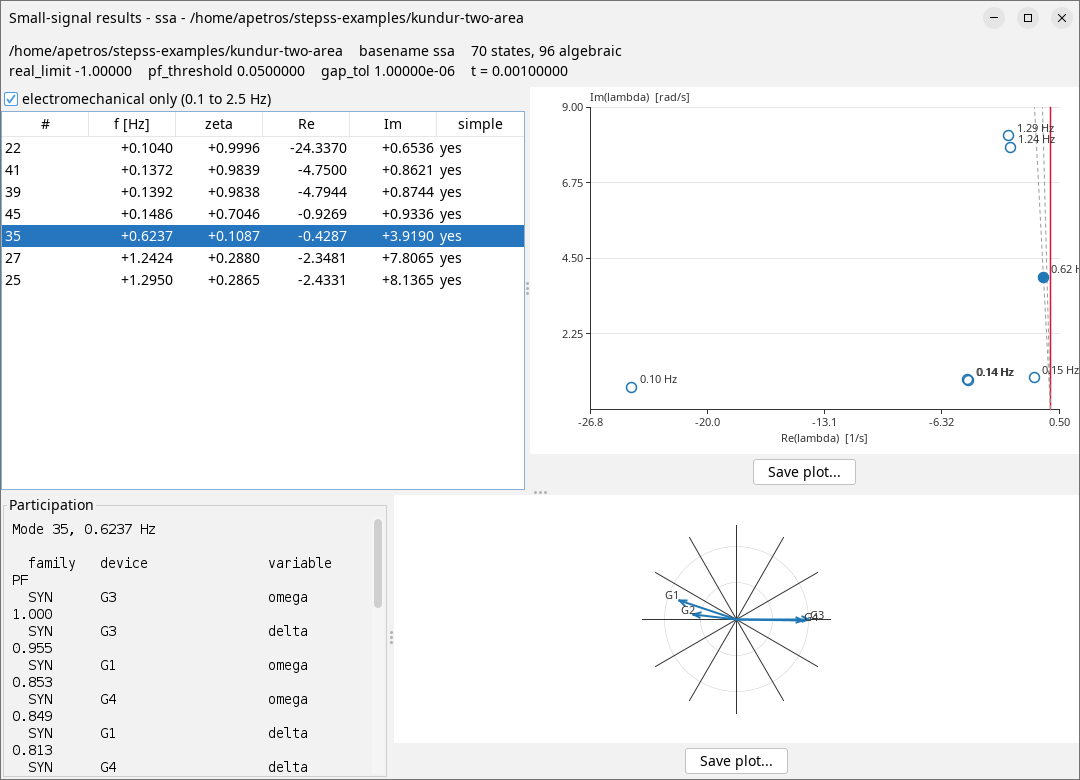
\includegraphics[width=0.98\linewidth]{figures/gui-ssa-results-light}
\caption{The small-signal results window for the Kundur case.}
\end{figure}

Reading that window across is the whole method in one view. The table gives the
frequency and damping of each mode; the s-plane shows how much margin each one
has, with the boundary drawn at the imaginary axis, so a mode crossing it is the
instability. Every mode is one circle there, crimson if it is unstable and
filled if it is the one selected. The \textbf{Participation} panel answers which
machines make up that mode, its last column \textbf{PF} being the participation
factor, normalised so the largest in each mode is 1. The mode shape answers how
those machines move relative to each other: here G1 and G2 swing against G3 and
G4, which is what makes 0.62 Hz the inter-area mode rather than a local one.

\subsection{Filtering and zooming}\label{eigenanalysis:filtering-and-zooming}

Three controls sit above the table, and all of them act on results already in
hand. Changing one re-filters what is on screen; none of them requires the
analysis to be run again.

\begin{small}\begin{longtable}[]{@{}
  >{\raggedright\arraybackslash}p{(\linewidth - 4\tabcolsep) * \real{0.3318}}
  >{\raggedright\arraybackslash}p{(\linewidth - 4\tabcolsep) * \real{0.6682}}
@{}}
\toprule\noalign{}
\begin{minipage}[b]{\linewidth}\raggedright
Control
\end{minipage} & \begin{minipage}[b]{\linewidth}\raggedright
What it does
\end{minipage} \\
\midrule\noalign{}
\endhead
\bottomrule\noalign{}
\endlastfoot
\textbf{electromechanical only} & Restricts to the 0.1 to 2.5 Hz band, where rotor-angle modes live. On by default \\
\textbf{real part above} & Hides modes at or below the value beside it. Off by default \\
\textbf{PF at least} & Trims the Participation panel to entries at or above the value beside it \\
\end{longtable}\end{small}

The count underneath says how many modes survive, so a filter that empties the
table reads as a filter rather than as a broken load.

\textbf{real part above} is the one that used to be the \texttt{real\_limit} parameter of the
run. It is worth reaching for on a full spectrum: this case is 70 states, most
of them fast controller and network dynamics that no rotor participates in, and
a handful of them sit far enough to the left to stretch the s-plane's real axis
until everything worth reading is squashed against the boundary. The plot refits
its axes whenever the filter changes, so hiding those modes closes the plane in
around what is left.

For a closer look than a filter gives, \textbf{drag a rectangle on the s-plane} to
zoom into it. \textbf{Reset zoom}, beside \textbf{Save plot\ldots{}}, goes back to the fitted
window, and double-clicking the plot does the same. A zoomed plot exports
zoomed: \textbf{Save plot\ldots{}} writes what is on screen, not the whole plane.

\begin{docsnote}{Note}

This screenshot is light in both site themes. The window itself follows the
application's theme from v3.74.20, plot panels included; before that release the
s-plane and the mode shape stayed white under the dark theme. A plot saved with
\textbf{Save plot\ldots{}} is drawn on white whatever theme is in use, since it is meant
for a report rather than the screen.

\end{docsnote}

\section{See Also}\label{eigenanalysis:see-also}

\begin{itemize}
\tightlist
\item
  \hyperref[ch-disturb]{Export Jacobian Matrix}, the
  \texttt{JAC} disturbance, for exporting the matrices instead of analysing them
\item
  \hyperref[doc:py-api]{\texttt{getJac()}}, the descriptor matrices as SciPy
  sparse objects, for driving your own solver
\item
  \hyperref[doc:ts-kundur]{Kundur Two-Area System}
\end{itemize}
